\section{Исследование и построение решения задачи}
\label{sec:Chapter3} \index{Chapter3}
С целью исследования и разработки своих собственных OSINT методов сбора информации о человеке с помощью поисковых сервисов и 
социальных сетей предстоит решить следующие задачи:
\begin{itemize}
    \item поисковые сервисы:
    \begin{enumerate}
        \item Определить структуру поискового сайта. В качестве таких сайтов возьмем следующие ресурсы:
        \begin{itemize}
            \item DuckDuckGo;
            \item Google;
            \item Yandex;
            \item Yahoo.
        \end{itemize}
        \item Извлечение найденных ссылок по заданному ключевому слову.
        \item Сбор информации с сайтов по отобранным ссылкам.
        \item Для случая с Google попробовать Google Search API: определить шаблон GET-запроса, структуру возвращаемых данных.
    \end{enumerate}
    \item социальные сети:
    \begin{enumerate}
        \item Определить структуру сайта социальной сети. Будем работать над социальной сетью LinkedIn.
        \item Реализовать поиск и сбор данных пользователей и организаций посредством веб-краулинга сайта.
        \item Реализовать сбор данных пользователей и организаций посредством закрытого API LinkedIn. Для этого потребуется:
        \begin{itemize}
            \item реализовать вход систему через закрытое API посредством GET и POST запросов;
            \item определить шаблон GET-запроса для получения данных по указанным ключевым словам, структуру возвращаемых данных.
        \end{itemize}
    \end{enumerate}
    \item реализовать все указанные выше подзадачи в систему сбора данных. 
\end{itemize}

\subsection{Исследование архитектуры сборщиков Scrapy}

Поскольку основным фреймворком для сбора данных является Scrapy, то необходимо изначально ознакомиться с его архитектурой.
\cite{scrapyArchitecture}

\begin{figure}[H]
    \center{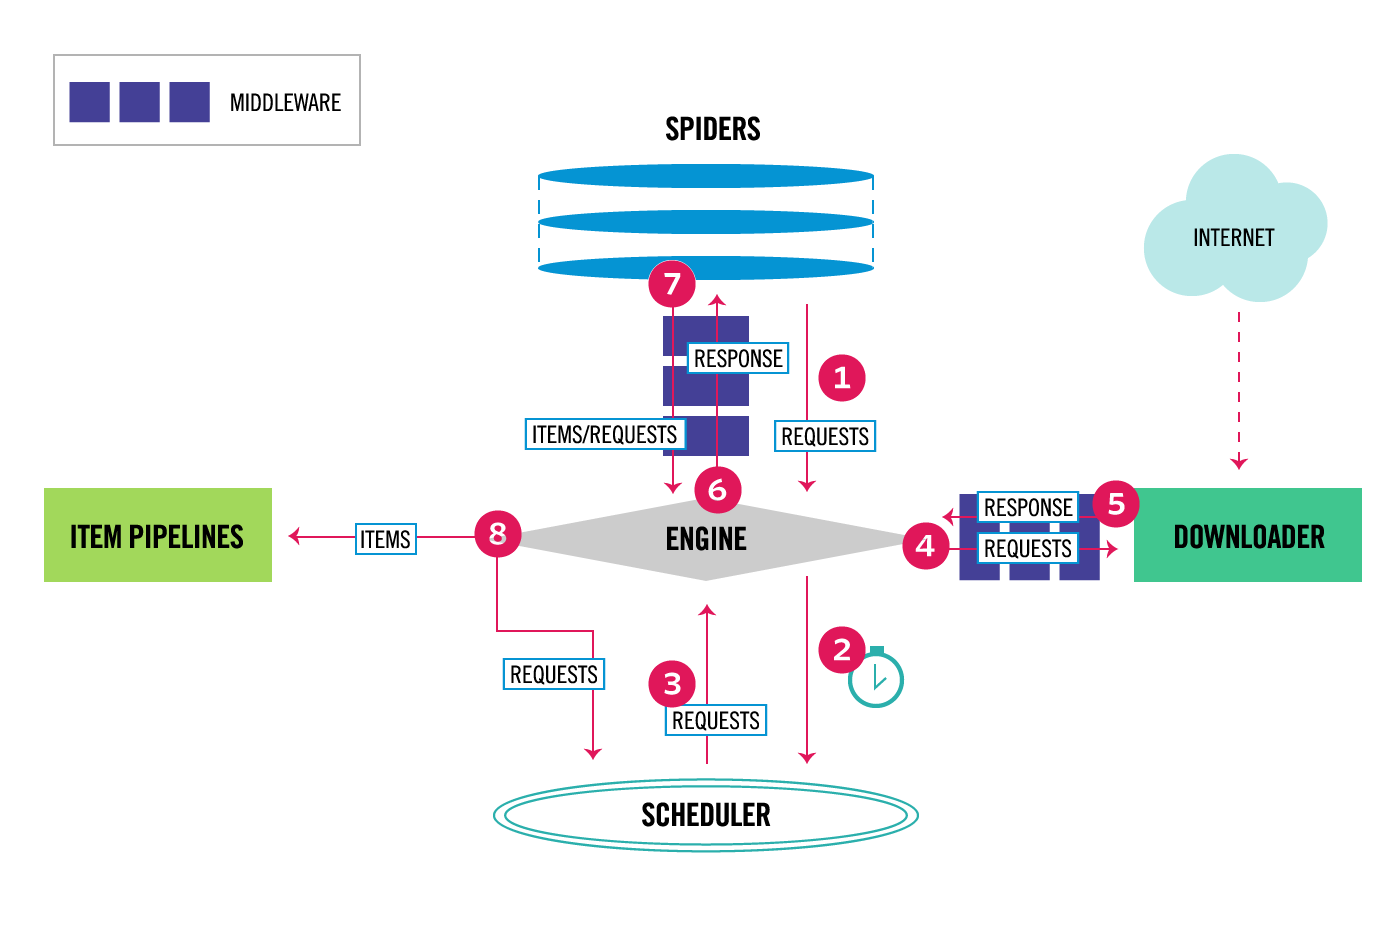
\includegraphics[height=6cm,keepaspectratio]{pictures/scrapy_architecture.png}}
    \caption{Архитектура Scrapy spider.}
    \label{ris:image}
\end{figure}

\par
Из рисунка видно, что изначально из spider'ов запросы направляются в движок и планировщик, затем через промежуточный загрузчик
запросы выполяются в сети Интернет. Ответ от ресурсов возвращается в загрузчик, оттуда обратно в движок и в конвейер элементов.
В нашей задаче потребуется писать собственные downloader middlewares и pipelines, помимо самих spiders непосредственно.

\subsubsection{Scrapy Downloader Middleware} 
Обусловленно это тем, что на этапе, когда запрос находится в загрузчике, есть возможность загрузить api-токен, логин и пароль,
или cookie-файлы для браузера и подставить его в запрос (переопределяемый метод process\_request). 
В случае, если учетных данных нет, то в загрузчике можно составить несколько вспомогательных запросов, которые нагенерируют 
новые cookie-файлы и подставят в исходный запрос. Также есть возможность обработать ответ в методе process\_response. 
Этот метод может использоваться для обновления учетных данных, кодов ответа, отличных от 200, но которые допустимы для запроса.
Стоит отметить, что каждый запрос, запущенный внутри проекта, будет проходить через process\_request и process\_response. Это
образует некую рекурсию и сложности для понимания, от какого именно запроса мы получили ответ.  

\subsubsection{Scrapy Item Pipelines}  
Изначально Scrapy просто собирает данные в некий массив структур, который можно выгрузить в json файл. Но фреймворк также 
поддерживает функционал скачивания файлов по их url. Для изображений используется встроенный ImagePipeline, для файлов --
FilesPipeline. Но есть потребность иногда рендерить веб-страницы полностью, так как Scrapy не поддерживает выполнение JavaScipt
файлов. Для рендера html страниц будем использовать Splash\footnote{https://splash.readthedocs.io/en/stable/} и фреймворк 
scrapy-splash\footnote{https://github.com/scrapy-plugins/scrapy-splash}. Таким образом, для выгрузки наибольшего количества
данных, документов и изображений с веб-страниц будет использовать SplashRequest, который вернет текст html-страницы с всеми
отработанными JavaScipt-скриптами.